\documentclass[]{article}
\usepackage{lmodern}
\usepackage{amssymb,amsmath}
\usepackage{ifxetex,ifluatex}
\usepackage{fixltx2e} % provides \textsubscript
\ifnum 0\ifxetex 1\fi\ifluatex 1\fi=0 % if pdftex
  \usepackage[T1]{fontenc}
  \usepackage[utf8]{inputenc}
\else % if luatex or xelatex
  \ifxetex
    \usepackage{mathspec}
  \else
    \usepackage{fontspec}
  \fi
  \defaultfontfeatures{Ligatures=TeX,Scale=MatchLowercase}
\fi
% use upquote if available, for straight quotes in verbatim environments
\IfFileExists{upquote.sty}{\usepackage{upquote}}{}
% use microtype if available
\IfFileExists{microtype.sty}{%
\usepackage{microtype}
\UseMicrotypeSet[protrusion]{basicmath} % disable protrusion for tt fonts
}{}
\usepackage[margin=1in]{geometry}
\usepackage{hyperref}
\hypersetup{unicode=true,
            pdftitle={Predicting Real Estate Sales Using Machine Learning and Spatial Dependence},
            pdfborder={0 0 0},
            breaklinks=true}
\urlstyle{same}  % don't use monospace font for urls
\usepackage{longtable,booktabs}
\usepackage{graphicx,grffile}
\makeatletter
\def\maxwidth{\ifdim\Gin@nat@width>\linewidth\linewidth\else\Gin@nat@width\fi}
\def\maxheight{\ifdim\Gin@nat@height>\textheight\textheight\else\Gin@nat@height\fi}
\makeatother
% Scale images if necessary, so that they will not overflow the page
% margins by default, and it is still possible to overwrite the defaults
% using explicit options in \includegraphics[width, height, ...]{}
\setkeys{Gin}{width=\maxwidth,height=\maxheight,keepaspectratio}
\IfFileExists{parskip.sty}{%
\usepackage{parskip}
}{% else
\setlength{\parindent}{0pt}
\setlength{\parskip}{6pt plus 2pt minus 1pt}
}
\setlength{\emergencystretch}{3em}  % prevent overfull lines
\providecommand{\tightlist}{%
  \setlength{\itemsep}{0pt}\setlength{\parskip}{0pt}}
\setcounter{secnumdepth}{0}
% Redefines (sub)paragraphs to behave more like sections
\ifx\paragraph\undefined\else
\let\oldparagraph\paragraph
\renewcommand{\paragraph}[1]{\oldparagraph{#1}\mbox{}}
\fi
\ifx\subparagraph\undefined\else
\let\oldsubparagraph\subparagraph
\renewcommand{\subparagraph}[1]{\oldsubparagraph{#1}\mbox{}}
\fi

%%% Use protect on footnotes to avoid problems with footnotes in titles
\let\rmarkdownfootnote\footnote%
\def\footnote{\protect\rmarkdownfootnote}

%%% Change title format to be more compact
\usepackage{titling}

% Create subtitle command for use in maketitle
\newcommand{\subtitle}[1]{
  \posttitle{
    \begin{center}\large#1\end{center}
    }
}

\setlength{\droptitle}{-2em}
  \title{Predicting Real Estate Sales Using Machine Learning and Spatial
Dependence}
  \pretitle{\vspace{\droptitle}\centering\huge}
  \posttitle{\par}
\subtitle{Boosting ML Predictive Accuracy Using Spatial Lags}
  \author{}
  \preauthor{}\postauthor{}
  \date{}
  \predate{}\postdate{}

\setlength{\parindent}{0em}
\setlength{\parskip}{1em}
\usepackage[fontsize=12pt]{scrextend}
\usepackage{fancyhdr}
\pagestyle{fancy}
\fancyhead[R]{\thepage}

\begin{document}
\maketitle

{
\setcounter{tocdepth}{2}
\tableofcontents
}
\newpage

\section{Introduction}\label{introduction}

In this paper, we explore a technique for more accurately predicting
real estate transactions, both their occurrence (probability of sale)
and their dollar amount (sale price per square foot). We explain how
this predictive technique may be applied to combat Economic Exclusion, a
precursor to Income Inequality. The technique marries the use of
machine-learning predictive models (Random Forrest) with ``spatial-lag''
features typically seen in geographically-weighted regressions (GWR). We
find that, while the addition of many new variables to a modeling data
set can inhibit the models' ability to generalize into the future,
spatial-lag features 1) consistently outperform zip-code level
aggregation features, and 2) outperform all models for specific types of
properties in specific areas. We conclude that spatial-lag features,
while computationally expensive, can be used to significantly increase
the predictive accuracy of spatial predictive models.

\subsection{What is Economic
Exclusion?}\label{what-is-economic-exclusion}

Income inequality may be a defining challenge of our time, yet the
causes of inequality remain unclear. As discussed by Zuk (2015),
``Neighborhoods change slowly, but over time {[}they{]} are becoming
more segregated by income, due in part to macro-level increases in
income inequality''. Researchers at the Urban Institute (Solomon Greene
and Lei 2016) recently identified the socio-economic phenomenon of
``Economic Exclusion'' as an explanation for income inequality in the
US. Economic Exclusion can be explained as follows: vulnerable
populations--disproportionately communities of color, immigrants,
refugees, and women--who are physically displaced by local economic
prosperity can enter into a gradual cycle of diminished access to good
jobs, good schools, health care facilities, public spaces, etc.
Diminished access leads to more poverty, which leads to more
displacement. Such self-reinforcing poverty gradually exacerbates income
inequality over the course years and even generations.

\subsection{Predicting Gentrification}\label{predicting-gentrification}

One practical way to combat Economic Exclusion is to focus on preventing
displacement, i.e., the physical relocation of populations away from
economic resources. As argued by Clay (1979), displacement is the
negative consequence of gentrification. Predicting gentrification at an
early stage, however, has proven to be a difficult task historically.
When an area experiences economic growth, increased housing demands and
subsequent affordability pressures can lead to voluntary or involuntary
relocation of low-income families and small businesses. Government
agencies and nonprofits tend to intervene once displacement is already
underway, and after-the-fact interventions can be costly and
ineffective. As explained by Solomon Greene and Lei (2016), there are
several preemptive actions that can be deployed to stem divestment and
ensure that existing residents benefit from new investments. Not unlike
medical treatment, early detection is the key to success. Consequently,
in 2016, the Urban Institute put forth a call for research into the
creation of ``neighborhood-level early warning and response systems that
can help city leaders and community advocates get ahead of neighborhood
changes'' (Solomon Greene and Lei 2016). This paper explores a technique
to answer that call in part.

\section{Literature Review}\label{literature-review}

We review Economic Displacement as it has been addressed in academia,
primarily in relation to the study of gentrification. We also examine
``mass appraisal techniques'', which are automated analytical techniques
used for valuing large numbers of real estate properties. Finally, we
will briefly examine machine learning as it relates to the problem of
predicting gentrification and/or Economic Displacement.

\subsection{How Has Economic Displacement Been Addressed in the
Past?}\label{how-has-economic-displacement-been-addressed-in-the-past}

Economic Displacement has been intertwined with the study of
gentrification since shortly after the latter became academically
relevant in the 1960's. The term ``gentrification'' was first used by
Ruth Glass in 1964 to described the ``gentry'' in low income
neighborhoods in London. Gentrification was originally understood as a
``tool of revitalization for declining neighborhoods'' (Zuk 2015),
however, in 1979 Phillip Clay made the distinction between two types of
revitalization: ``incumbent upgrading'' and ``gentrification'', noting
that Economic Displacement was the negative consequence of the latter
(Clay 1979). Today, the term has evolved to describe ``a spatial
organization and re-organization of human dwelling and activity'' (Zuk
2015). Specific to cities, gentrification is thought of as ``the
transformation of a working-class or vacant area of the central city
into middle-class residential or commercial use'' (Lees 2008).

Studies of gentrification and displacement generally take two approaches
in the literature: supply-side and demand-side, or ``the flows of
capital versus flows of people to neighborhoods'', respectively (Zuk
2015). Supply side arguments for gentrification tend to focus on
``private capital investment, public policies, and public investments''
(Zuk 2015). Smith (1979) argued that the return of capital from the
suburbs to the city drives gentrification. He describes a ``political
economy of capital flows into urban areas'' as largely responsible for
both the positive and negative consequences of gentrification. According
to Dreier (2004), public policies that have been linked to increased
Economic Displacement have been, among others, automobile-oriented
transportation infrastructure spending and mortgage interest tax
deductions for home owners.

More recently, income inequality has been explored as a consequence of
Economic Displacement, defined as ``higher compensation in the top
quintile and the lack of jobs for the bottom quintile'' (Reardon 2011);
(Watson 2009). The concentration of wealth allows ``certain households
to sort themselves according to their preferences -- and control local
political processes that continue exclusion'' (Reardon 2011). This
results in a self-reinforcing feedback loop where wealthier households
influence public policy toward their self interest. Gentrification
prediction tools could be used to help break such feedback loops through
early identification and intervention.

Many studies conclude that gentrification in most forms leads to
Economic Displacement, however, Zuk (2015) characterizes the results of
many recent studies as ``mixed, due in part to methodological
shortcomings''. In this paper, we attempt to further the understanding
of gentrification prediction by demonstrating a technique to better
predict real estate sales in New York City.

\subsection{A Review of Mass Appraisal
Techniques}\label{a-review-of-mass-appraisal-techniques}

Much of the research on predicting real estate transaction has been in
service of ``mass appraisal'' models, or models that are used to value
large numbers of buildings automatically. Such techniques are commonly
used by governments for the purposes of collecting taxes from property
owners. Mass appraisal models share many characteristics with predictive
machine learning models (and are not mutually exclusive), in that they
are data-driven, standardized methods that employ statistical testing
(Eckert 1990). A variation on mass appraisal models are the ``automated
valuation models'' (AVM), which use ``often the same methodological
framework of mass appraisal\ldots{} a statistical model and a large
amount of property data to estimate the market value of an individual
property or portfolio of properties'' (d'Amato 2017).

Scientific mass appraisal models date back to 1936 with the reappraisal
of St.~Paul, Minnesota (Silverherz 1936). Since that time, and
accelerated with the advent of computers, much statistical research has
been done relating property values and rent prices to various
characteristics of those properties, including characteristics of their
surrounding areas. Multiple regression analysis (MRA) has been the most
common set of statistical tools used in mass appraisal, including
Maximum Likelihood, Weighted Least Squares, and the most popular,
Ordinary Least Squares (OLS) (d'Amato 2017). The primary drawbacks of
MRA techniques are ``excessive multicollinearity among attributes'' and
``spatial autocorrelation among residuals'' (d'Amato 2017). Another
group of models that seek to correct for spatial dependence are known as
Spatial Auto Regressive (SAR) models, chief among them the Spatial Lag
Model, which aggregates weighted summaries of nearby properties in order
to create independent regression variables (d'Amato 2017). Geographic
Weighted Regressions frequently employ spatial lags.

Hedonic regression modeling is the practice of defining and quantifying
the components of a price of a good based on the intrinsic and extrinsic
characteristics. Koschinsky (2012) is a recent and thorough discussion
of parametric hedonic regression techniques. Some of the variables
included in Koschinsky's models are derived from nearby properties,
similar to the technique used in this paper, and these variables were
found to be predictive. The real estate hedonic model as defined by
Koschinsky describes the price of a property as:

\[
\begin{aligned}
 P_i = P(S_i, N_i, L_i)
\end{aligned}
\]

Where \(P_i\) represents the price of house \(i\), which is a composite
good comprised of a vector of structural characteristics \(S\), a vector
of social and neighborhood characteristics \(N\), and a vector of
locational characteristics \(L\). The model calculates spatial lags for
properties of interest using neighboring properties within 1,000 feet of
a sale. The derived variables include characteristics such as average
age, quantity of poor condition homes nearby, percent of homes with
electric heating nearby, construction grade, etc. Koschinsky found that
in all cases, ``the relation between a home's price and the average
price of its neighboring homes is characterized by positive spatial
autocorrelation'' meaning that homes near each other were typically
similar to each other and priced accordingly. Koschinsky concluded that
locational characteristics should be valued at least as much ``if not
more'' than structural characteristics.

As recently as 2015, much research has dealt with mitigating the
drawbacks of spatial multiple regression analysis through the use of
multi-level hierarchical models. Fotheringham (2015) explored the
combination of Geographically Weighted Regression (GWR) with time-series
forecasting to predict home prices over time. He used ``adaptive
bandwidths'' of local data, i.e., for each estimate, the number of data
points included varied was optimized using cross-validation. Adaptive
bandwidths are an interesting extension to spatial lag models and are
included in the ``Future Research'' portion of this paper.

Automated valuation modeling got a legal update in the aftermath of the
2008 financial crisis by way of the The Dodd Frank Act. In particular,
the Title XIV, subtitle F distinguishes the ``appraisal'' process from
automated valuation modelling, and reorganized both (d'Amato 2017). The
Act asserts that appraisal, or valuation conducted by a human being,
cannot be replaced by AVM. At current, AVM is ``increasingly adaptable
in describing real estate market behavior'' but has yet to supersede the
importance and necessity of local information and human evaluation.

\subsection{Has Machine Learning Been Applied to this Problem
Before?}\label{has-machine-learning-been-applied-to-this-problem-before}

Both Mass Appraisal techniques and Automated Valuation Modeling seek to
predict real estate prices using data and statistical methods, however,
traditional techniques typically fall short of reality. This is because
property valuation is inherently a ``chaotic'' process that does not
lend itself to binary or linear analysis (Zuk 2015). The value of any
given property is a complex combination of perceived value and
speculation. The value of any building or plot of land belongs to a rich
network where decisions about and perceptions of neighboring properties
influence the final market value. Guan et al. (2014) compared
traditional MRA techniques to alternative ``data mining techniques''
resulting in ``mixed results''. However, as Helbich (2013) states,
hedonic pricing models ``can be improved in two ways: (a) Through novel
estimation techniques, and (b) by ancillary structural, locational, and
neighborhood variables on the basis of Geographic Information System
(GIS)''. Recent research generally falls into these two buckets: better
analysis algorithms and/or better data.

In the ``better data'' category, researchers have been striving to
introduce new independent variables to increase the accuracy of
predictive models. Dietzell (2014) successfully used internet search
query data provided by Google Trends to serve as a sentiment indicator
and improve commercial real estate forecasting models. Pivo and Fisher
(2011) examined the effects of walkability on property values and
investment returns. They found that on a 100-point scale, a 10-point
increase in walkability increased property investment values by up to
9\%.

Research into better prediction algorithms do not necessarily happen at
the exclusion of ``better data''. For example, Fu (2014) created a
prediction algorithm, called ``ClusRanking'', for real estate in
Beijing, China. ClusRanking first estimates neighborhood characteristics
using taxi cab traffic vector data, specifically as they relate to
nearby ``business areas''. Subsequently, the algorithm performs a
rank-ordered prediction of investment returns segmented into five
categories. Similar to Koschinsky (2012), though less formally stated,
Fu (2014) thought of a property's value as a composite of individual,
peer and zone characteristics. In the predictive model, Fu includes
characteristics of the neighborhood (individual), the values of its
nearby properties (peer), and the prosperity of the affiliated latent
business area (zone) based on taxi cab data (Fu 2014).

Several other recent studies compare various ``advanced'' statistical
techniques and algorithms either to other advanced techniques or to
traditional ones. Most studies conclude that the advanced,
non-parametric techniques outperform traditional parametric techniques,
while several conclude that the Random Forest algorithm is particularly
well-suited to predicting real estate values.

Kontrimasa (2011) compares the accuracy of linear regression against the
SVM technique and found the latter to outperform. Schernthanner H.
(2016) compared traditional linear regression techniques to several
techniques such as krigging (stochastic interpolation) and Random
Forest. They concluded that the more advanced techniques, particularly
Random Forest, are sound and more accurate when compared to traditional
statistical methods. Antipov and Pokryshevskaya (2012) comes to a
similar conclusion about the superiority of Random Forest to real estate
valuation after comparing 10 algorithms: multiple regression, CHAID,
Exhaustive CHAID, CART, 2 types of k-Nearest Neighbors, Multilayer
Perceptron neural network (MLP), Radial Basis Function neural network
(RBF)), Boosted Trees and finally Random Forest.

Guan et al. (2014) compared three different approaches to defining
spatial neighbors: a simple radius technique, a k-nearest neighbors
technique (KNN) using only distance and a KNN technique using all
attributes. Interestingly, the location-only KNN models performed best,
although by a slight margin. Park (2015) developed several housing price
prediction models based on machine learning algorithms including C4.5,
RIPPER, Naive Bayesian, and AdaBoost. By comparing the models'
classification accuracy performance, the experiments demonstrate that
the RIPPER algorithm, based on accuracy, consistently outperformed the
other models in the performance of housing price prediction. Rafiei
(2016) employed a restricted boltzmann machine (neural network with back
propagation) to predict the sale price of residential condos in Tehran,
Iran. Rather than focusing on predictive performance, their paper
focuses on computational efficiency by employing ``a non-mating genetic
algorithm'' for dimensionality reduction. The paper concludes that two
primary strategies help in this regard: weighting property sales by
temporal proximity (sales which happened closer in time are more
important), and also using a learner to accelerate the recognition of
important features. The paper compares this technique to several other
common neural network approaches and finds that while not necessarily
the only way to get the best answer, it is the fastest way to get to the
best answer.

Finally, it should be noted that many studies, whether exploring
advanced techniques, new data, or both, rely on aggregation of data by
some arbitrary boundary. For example, Turner and Snow (2001) predicted
gentrification in the Washington, D.C. metro area by ranking census
tracts in terms of development. K. Chapple (2009) created a
gentrification ``early warning system'' by identifying low income census
tracts in central city locations. Barry Bluestone \& Chase Billingham
(2010) analyzed 42 census block groups near rail stations in 12 metro
areas across the United States, studying changes between 1990 and 2000
for neighborhood socioeconomic and housing characteristics. All of these
studies, and many more, relied on aggregation of data at the
census-tract or census-block level. In contrast, this paper compares
boundary-aggregation techniques (specifically, aggregating by zip codes)
to spatial-lag features and finds the spatial lag techniques to
consistently outperform.

\section{Methodology}\label{methodology}

Predictive modeling using spatial dependence has been employed
extensively in recent years, notably in Crime Prediction (Almanie 2015).
However, a key deficiency of many spatial models are their use of
arbitrarily defined geographic regions, such as zip codes, political
districts, police precincts, state lines, neighborhoods, etc., which
potentially diminish and obscure valuable insights. Worse yet, many
predictive models ignore spatial dependence, violating one of the basic
tenets of geography: the direct relationship between distance and
likeness (Miller 2007).

Our goal is to compare the use of spatial lags as features in a machine
learning predictive model against traditional feature engineering
techniques. We will create three modeling data sets:

\begin{itemize}
\tightlist
\item
  Base
\item
  Zip Code
\item
  Spatial Lag
\end{itemize}

We will then create 2 predictive models for each modeling data set,
using a different outcome variable for each:

\begin{enumerate}
\def\labelenumi{\arabic{enumi})}
\tightlist
\item
  Probability of Sale. The probability that a given property in New York
  City will sell in a given year
\item
  Amount of Sale. Given that a property sells, how much is the sale
  value?
\end{enumerate}

There will be six predictive models built in total, as follows:

\begin{longtable}[]{@{}lllllll@{}}
\caption{Six Predictive Models}\tabularnewline
\toprule
\# & Model & Model Type & Data & Outcome Var & Outcome Type & Eval
Metric\tabularnewline
\midrule
\endfirsthead
\toprule
\# & Model & Model Type & Data & Outcome Var & Outcome Type & Eval
Metric\tabularnewline
\midrule
\endhead
1 & Probability of Sale & Classification & Base & Building Sold & Binary
& AUC\tabularnewline
2 & Probability of Sale & Classification & Zip Code & Building Sold &
Binary & AUC\tabularnewline
3 & Probability of Sale & Classification & Spatial Lag & Building Sold &
Binary & AUC\tabularnewline
4 & Sale Price & Regression & Base & Sale Price per SF & Continuous &
RMSE\tabularnewline
5 & Sale Price & Regression & Zip Code & Sale Price per SF & Continuous
& RMSE\tabularnewline
6 & Sale Price & Regression & Spatial Lag & Sale Price per SF &
Continuous & RMSE\tabularnewline
\bottomrule
\end{longtable}

To accomplish this, we combine three open-source data repositories
provided by New York City via \url{nyc.gov} and
\url{data.cityofnewyork.us}. Our base modeling data set includes all
building records and associated sales information from 2003-2017.

Following the creation of the base modeling data, we create two
additional data sets through feature engineering: a ``Zip Code
features'' data set and a ``Spatial Lag features'' data set. The primary
goal of this study is to compare the predictive power of the spatial
lags vs.~the base and zip code features. We will seek to predict sales
one year into the future by training and validating on 2003-2016 data
and making predictions on 2017 data.

\subsection{Data}\label{data}

The New York City government makes available an annual data set which
describes all tax lots in the five boroughs. The Primary Land Use and
Tax Lot Output data set, known as
\href{https://www1.nyc.gov/site/planning/data-maps/open-data/bytes-archive.page?sorts\%5Byear\%5D=0}{PLUTO},
contains a single record for every tax lot in the city along with a
number of building and tax-related attributes such as Year Built,
Assessed Value, Square Footage, number of stories, and many more. At the
time of this writing, NYC has made this data set available for all years
between 2002-2017, excluding 2008. For convenience, we also exclude the
2002 data set from our analysis because sales information is not
available for that year. Importantly for our analysis, the latitude and
longitude of the tax lots are also made available, allowing us to locate
in space each building and to build geospatial features from the data.

Ultimately, we are interested in sales transactions--both frequency, and
amount. Sales transactions are also made available by the New York City
government, known as
\href{http://www1.nyc.gov/site/finance/taxes/property-annualized-sales-update.page}{NYC
Rolling Sales Data}. At the time of this writing, sales transactions are
available for the years 2003-2017. The sales transactions data contains
additional data fields describing time, place, and amount of sale as
well as additional building characteristics. Crucially, the sales
transaction data does not include geographical coordinates, making it
impossible to perform geospatial analysis without first mapping the
sales data to PLUTO.

Prior to mapping to PLUTO, the sales data must first be transformed to
include the proper mapping key. New York City uses a standard key of
Borough-Block-Lot to identify tax lots in the data. For example, 31 West
27th Street is located in Manhattan, on block 829 and lot 16, therefore,
its Borough-Block-Lot (BBL) is 1\_829\_16 (the 1 represents Manhattan).
The sales data contain BBL's at the building level, however, the sales
transactions data does not appropriately differentiate condos as their
own BBL's. Mapping the sales data directly to the PLUTO data results in
a mapping error rate of 23.1\%. Therefore, the sales transactions data
must first be mapped to another data source, the NYC Property Address
Directory, or
\href{https://data.cityofnewyork.us/City-Government/Property-Address-Directory/bc8t-ecyu/data}{PAD},
which contains an exhaustive list of all BBL's in NYC. Once the sales
data is combined with PAD, the data can be mapped to PLUTO with an error
rate of just 0.291\%.

Prior to mapping, the sales data are normalized and filtered so that
only BBL's with less than or equal to 1 transactions in a year occur.
The final data set is an exhaustive list of all tax lots in NYC for
every year between 2003-2017, whether that building was sold, for what
amount, and several other variables.

Several building categories are excluded from the data for ease of
modeling and subsequent analysis. The following building types are
included:

\begin{longtable}[]{@{}ll@{}}
\caption{Building Types Included in Modeling Data}\tabularnewline
\toprule
Building Type & Description\tabularnewline
\midrule
\endfirsthead
\toprule
Building Type & Description\tabularnewline
\midrule
\endhead
A & ONE FAMILY DWELLINGS\tabularnewline
B & TWO FAMILY DWELLINGS\tabularnewline
C & WALK UP APARTMENTS\tabularnewline
D & ELEVATOR APARTMENTS\tabularnewline
F & FACTORY AND INDUSTRIAL BUILDINGS\tabularnewline
G & GARAGES AND GASOLINE STATIONS\tabularnewline
L & LOFT BUILDINGS\tabularnewline
O & OFFICES\tabularnewline
\bottomrule
\end{longtable}

The data is further filtered to include only records with equal to or
less than 2 buildings per tax lot. The global filtering of the data set
reduces the base modeling data from 12,012,780 records down to
8,247,499.

\subsection{Feature Engineering}\label{feature-engineering}

\subsubsection{Base modeling data}\label{base-modeling-data}

The base modeling data--a combination of PLUTO, PAD and Rolling Sales--
are enhanced with additional features. A summary table of the additional
features are presented below:

\begin{longtable}[]{@{}lllll@{}}
\caption{Base Modeling Data Features}\tabularnewline
\toprule
Feature & Min & Median & Mean & Max\tabularnewline
\midrule
\endfirsthead
\toprule
Feature & Min & Median & Mean & Max\tabularnewline
\midrule
\endhead
has building area & 0 & 1.00 & 1.00 & 1.00\tabularnewline
Percent Com & 0 & 0.00 & 0.16 & 1.00\tabularnewline
Percent Res & 0 & 1.00 & 0.82 & 1.00\tabularnewline
Percent Office & 0 & 0.00 & 0.07 & 1.00\tabularnewline
Percent Retail & 0 & 0.00 & 0.04 & 1.00\tabularnewline
Percent Garage & 0 & 0.00 & 0.01 & 1.00\tabularnewline
Percent Storage & 0 & 0.00 & 0.02 & 1.00\tabularnewline
Percent Factory & 0 & 0.00 & 0.00 & 1.00\tabularnewline
Percent Other & 0 & 0.00 & 0.00 & 1.00\tabularnewline
Last Sale Price & 0 & 312.68 & 531.02 & 62,055.59\tabularnewline
Last Sale Price Total & 2 & 2,966,835.00 & 12,844,252.00 &
1,932,900,000.00\tabularnewline
Years Since Last Sale & 1 & 4.00 & 5.05 & 14.00\tabularnewline
SMA Price 2 year & 0 & 296.92 & 500.89 & 62,055.59\tabularnewline
SMA Price 3 year & 0 & 294.94 & 495.29 & 62,055.59\tabularnewline
SMA Price 5 year & 0 & 300.12 & 498.82 & 62,055.59\tabularnewline
Percent Change SMA 2 & -1 & 0.00 & 685.69 & 15,749,999.50\tabularnewline
Percent Change SMA 5 & -1 & 0.00 & 337.77 & 6,299,999.80\tabularnewline
EMA Price 2 year & 0 & 288.01 & 482.69 & 62,055.59\tabularnewline
EMA Price 3 year & 0 & 283.23 & 471.98 & 62,055.59\tabularnewline
EMA Price 5 year & 0 & 278.67 & 454.15 & 62,055.59\tabularnewline
Percent Change EMA 2 & -1 & 0.00 & 422.50 & 9,415,128.85\tabularnewline
Percent Change EMA 5 & -1 & 0.06 & 308.05 & 5,341,901.60\tabularnewline
\bottomrule
\end{longtable}

A binary variable is created to indicate whether a tax lot has a
building on it (i.e., whether it is an empty plot of land or not). In
addition, building types are quantified by what percent of the square
footage belongs to the major property types: Commercial, Residential,
Office, Retail, Garage, Storage, Factory and Other.

Importantly, two variables are created from the Sales Prices: A
price-per-square-foot figure (``Last Sale Price'') and a total Sale
Price (``Last Sale Price Total''). Sale Price per Square foot eventually
becomes the outcome variable in one of the predictive models, even
though it is referred to as Sale Price. Further features are derived
which carry forward the previous sale price of a tax lot, if there is
one, through successive years. Previous Sale Price is then used to
create Simple Moving Averages (SMA), Exponential Moving Averages (SMA),
and percent change measurements between the moving averages. In total,
69 variables are input to the feature engineering process and 92
variables are output. The final base modeling data set is 92 variables
by 8,247,499 rows.

\subsubsection{Zip Code Modeling Data}\label{zip-code-modeling-data}

The first of the comparative modeling data sets is the Zip code modeling
data. Using the base data as a starting point, several features are
created to describe characteristics of the zip code where the tax lot
resides. A summary table of the Zip code level features is presented
below. Note that ``bt only'' stands for ``Building Type only'' and
refers to aggregations that only include buildings of the same type as
the tax lot in question.

\begin{longtable}[]{@{}lll@{}}
\caption{Zip Code Modeling Data Features (continued
below)}\tabularnewline
\toprule
Feature & Min & Median\tabularnewline
\midrule
\endfirsthead
\toprule
Feature & Min & Median\tabularnewline
\midrule
\endhead
Last Year Zip Sold & 0.00 & 27.00\tabularnewline
Last Year Zip Sold Percent Ch & -1.00 & 0.00\tabularnewline
Last Sale Price zip code average & 0.00 & 440.95\tabularnewline
Last Sale Price Total zip code average & 10.00 &
5,312,874.67\tabularnewline
Last Sale Date zip code average & 12,066.00 & 13,338.21\tabularnewline
Years Since Last Sale zip code average & 1.00 & 4.84\tabularnewline
SMA Price 2 year zip code average & 34.31 & 429.26\tabularnewline
SMA Price 3 year zip code average & 34.31 & 422.04\tabularnewline
SMA Price 5 year zip code average & 39.48 & 467.04\tabularnewline
Percent Change SMA 2 zip code average & -0.20 & 0.04\tabularnewline
Percent Change SMA 5 zip code average & -0.09 & 0.03\tabularnewline
EMA Price 2 year zip code average & 30.77 & 401.43\tabularnewline
EMA Price 3 year zip code average & 33.48 & 419.11\tabularnewline
EMA Price 5 year zip code average & 29.85 & 431.89\tabularnewline
Percent Change EMA 2 zip code average & -0.16 & 0.06\tabularnewline
Percent Change EMA 5 zip code average & -0.08 & 0.07\tabularnewline
Last Sale Price bt only & 0.00 & 357.71\tabularnewline
Last Sale Price Total bt only & 10.00 & 3,797,461.46\tabularnewline
Last Sale Date bt only & 12,055.00 & 13,331.92\tabularnewline
Years Since Last Sale bt only & 1.00 & 4.78\tabularnewline
SMA Price 2 year bt only & 0.00 & 347.59\tabularnewline
SMA Price 3 year bt only & 0.00 & 345.40\tabularnewline
SMA Price 5 year bt only & 0.00 & 372.30\tabularnewline
Percent Change SMA 2 bt only & -0.55 & 0.03\tabularnewline
Percent Change SMA 5 bt only & -0.33 & 0.02\tabularnewline
EMA Price 2 year bt only & 0.00 & 332.98\tabularnewline
EMA Price 3 year bt only & 0.00 & 332.79\tabularnewline
EMA Price 5 year bt only & 0.00 & 340.57\tabularnewline
Percent Change EMA 2 bt only & -0.47 & 0.06\tabularnewline
Percent Change EMA 5 bt only & -0.34 & 0.06\tabularnewline
\bottomrule
\end{longtable}

\begin{longtable}[]{@{}ll@{}}
\toprule
Mean & Max\tabularnewline
\midrule
\endhead
31.14 & 112.00\tabularnewline
Inf & Inf\tabularnewline
522.87 & 1,961.21\tabularnewline
11,877,688.55 & 1,246,450,000.00\tabularnewline
13,484.39 & 17,149.00\tabularnewline
4.26 & 11.00\tabularnewline
501.15 & 2,092.41\tabularnewline
496.47 & 2,090.36\tabularnewline
520.86 & 2,090.36\tabularnewline
616.47 & 169,999.90\tabularnewline
341.68 & 113,333.27\tabularnewline
479.38 & 1,883.81\tabularnewline
479.95 & 1,781.38\tabularnewline
472.80 & 1,506.46\tabularnewline
388.90 & 107,368.37\tabularnewline
326.17 & 107,368.38\tabularnewline
485.97 & 6,401.01\tabularnewline
11,745,130.56 & 1,246,450,000.00\tabularnewline
13,497.75 & 17,149.00\tabularnewline
4.30 & 14.00\tabularnewline
462.67 & 5,519.39\tabularnewline
458.50 & 5,104.51\tabularnewline
481.09 & 4,933.05\tabularnewline
600.10 & 425,675.69\tabularnewline
338.15 & 188,888.78\tabularnewline
442.79 & 5,103.51\tabularnewline
443.02 & 4,754.95\tabularnewline
436.70 & 4,270.37\tabularnewline
377.17 & 254,462.97\tabularnewline
335.17 & 178,947.30\tabularnewline
\bottomrule
\end{longtable}

In general, the base model data features are aggregated to a zip code
level and attached to the individual observations, including SMA and EMA
calculations. Additionally, a second set of features are added, denoted
as ``bt only'', which filter only for tax lots of the same building
type. In total, the Zip code feature engineering process inputs 92
variables and outputs 122 variables.

\subsubsection{Spatial Lag modeling
data}\label{spatial-lag-modeling-data}

Spatial lags are variables created from physically proximate
observations, where the aggregations can be weighted by an arbitrary
distance function. For example, taking the average building age from all
buildings within 100 meters of the tax lot in question weighted by
inverse euclidean distance would constitue a spatial lag. A spatial lag
is defined as:

\[
(\rho)W_y + X(\beta)
\]

Where \(W_y\) is a spatially lagged dependent variable with weights
matrix \(W\), \(X\) is a matrix of observations on the explanatory
variable, and \(\rho\) and \(\beta\) are coeficients.

Creating spatial lags presents both advantages and disadvantages in the
modeling process. Spatial lags allow for a much more fine-tuned
measurement of a building's surrounding area. Knowing the average sale
price of all buildings within 500 meters of a building can be much more
informative than knowing the sale prices of all buildings in the same
zip code (but not always). However, building spatial lags is
computationally expensive. Each observation must be compared against
every other observation in the data set to determine which points fall
within the spatial lag radius and which do not. This can be
conceptualized in Big O notation as:

\[
O(n^n)
\]

To build spatial lags for all 8,247,499 observations in our modeling
data employed a novel spatial indexing technique to sped up the process.
Since tax lots rarely move from year to year, we reduced the indexing
task to 514,124 points (the number of unique tax lots in New York City).
We then partitioned the dataset into an arbitrary number of grids and
calculated spatial lags in parallel, assigning one grid to each
processing unit until the task was complete. By supplying a sufficiently
large number of processing units \(p\), the computation time can be
reduced to:

\[
O(n^\frac{n}{p})
\]

For each point in the dataset, we calculated and cached every other tax
lot within 500 meters of that building. The result was an
origin-destination relationship graph that related each tax lot to its
surrounding tax lots.

\begin{figure}
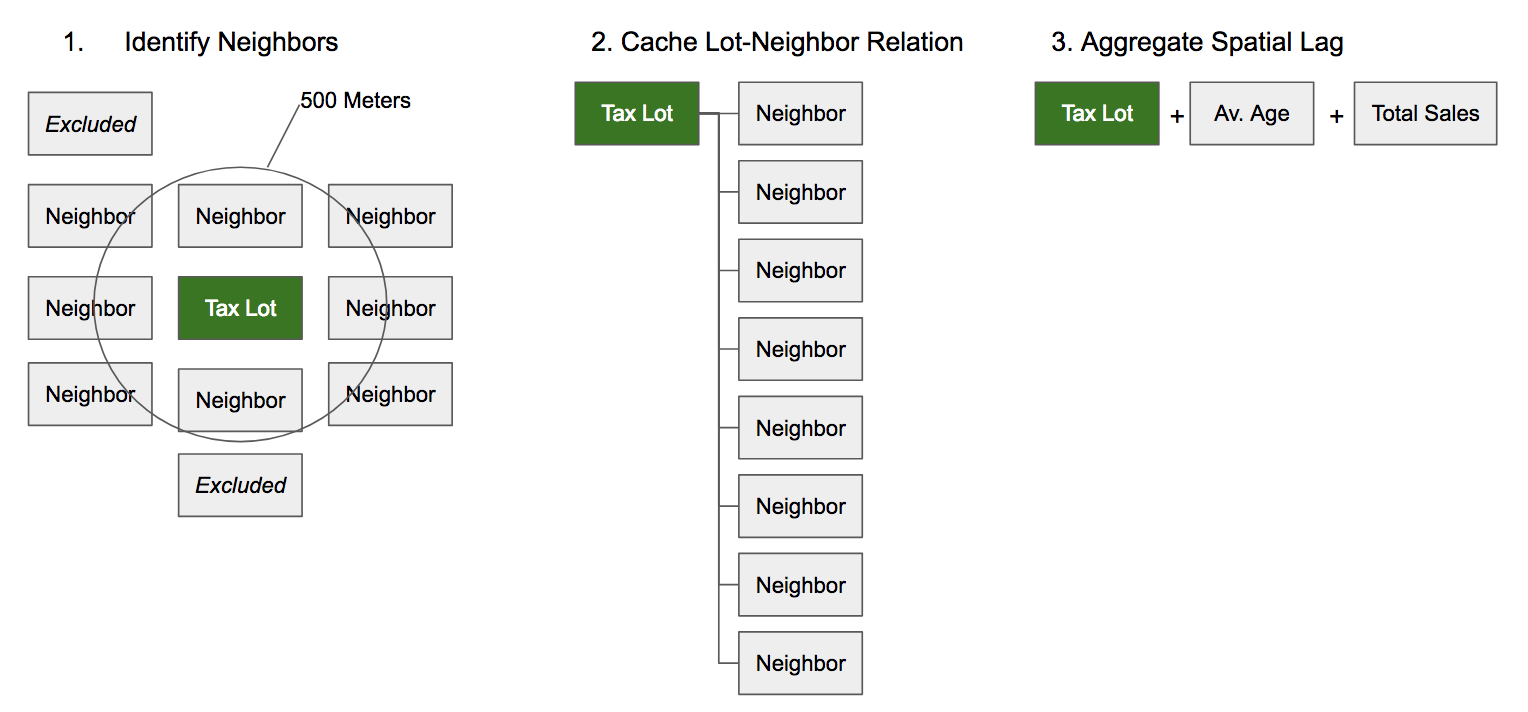
\includegraphics[width=1\linewidth]{Sections/tables and figures/Spatial Lag Creation} \caption{Illustrastion of Spatial Lag Creation}\label{fig:Spatial Lag Creation}
\end{figure}

Next, we used the spatial index to create spatial lag features (For an
illustration, see Figure \ref{fig:Spatial Lag Creation}). One advantage
to using spatial lags is the rich number of potential features which can
be created. Spatial lags can be weighted based on an arbitrary distance
function, e.g., physically closer observations can be given more weight.
For our modeling purposes, we created two sets of spatially weighted
features: distance weighted features (denoted with a ``\_dist``) and
simple average features (denoted with''\_basic``). SMA and EMA as well
as percent changes were also calculated. In total, the spatial lag
feature engineering process input 92 variables and output 194 variables.
A summary of the Spatial Lag features are presented in Table 6.

\begin{longtable}[]{@{}l@{}}
\caption{Summary of Spatial Lag Features}\tabularnewline
\toprule
Spatial Lag Features\tabularnewline
\midrule
\endfirsthead
\toprule
Spatial Lag Features\tabularnewline
\midrule
\endhead
Radius Total Sold In Year\tabularnewline
Radius Average Years Since Last Sale\tabularnewline
Radius Res Units Sold In Year\tabularnewline
Radius All Units Sold In Year\tabularnewline
Radius SF Sold In Year\tabularnewline
Radius Total Sold In Year sum over 2 years\tabularnewline
Radius Average Years Since Last Sale sum over 2 years\tabularnewline
Radius Res Units Sold In Year sum over 2 years\tabularnewline
Radius All Units Sold In Year sum over 2 years\tabularnewline
Radius SF Sold In Year sum over 2 years\tabularnewline
Radius Total Sold In Year percent change\tabularnewline
Radius Average Years Since Last Sale percent change\tabularnewline
Radius Res Units Sold In Year percent change\tabularnewline
Radius All Units Sold In Year percent change\tabularnewline
Radius SF Sold In Year percent change\tabularnewline
Radius Total Sold In Year sum over 2 years percent change\tabularnewline
Radius Average Years Since Last Sale sum over 2 years percent
change\tabularnewline
Radius Res Units Sold In Year sum over 2 years percent
change\tabularnewline
Radius All Units Sold In Year sum over 2 years percent
change\tabularnewline
Radius SF Sold In Year sum over 2 years percent change\tabularnewline
\bottomrule
\end{longtable}

Temporal and spatial derivatives of the Spatial Lag features presented
in Table 6 are also added to the model, including: variables weighted by
euclidean distance (``dist''), basic averages of the spatial lag radius
(``basic mean''), Simple Moving Averages (``SMA'') for 2 years, 3 years
and 5 years, exponential moving averages (``EMA'') for 2 years, 3 years
and 5 years, and year-over-year percent changes for all variables
(``perc change''). For a complete list of Spatial Lag features, see
Appendix A.

\subsection{Outcome Variables}\label{outcome-variables}

The final step in creating the modeling data is to define the outcome
variables. For our purposes, we create two dependent variables:

\begin{itemize}
\tightlist
\item
  Sold. Whether a tax lot sold in a given year. Used in the Probability
  of Sale classification model.
\item
  Sale Price. The price-per-square foot associated with a transaction,
  if a sale took place. Used in the Sale Price Regression model.
\end{itemize}

The following table describes the distributions of both outcome
variables:

\begin{longtable}[]{@{}lll@{}}
\caption{Distributions for Outcome Variables}\tabularnewline
\toprule
& Sold & Sale Price per SF\tabularnewline
\midrule
\endfirsthead
\toprule
& Sold & Sale Price per SF\tabularnewline
\midrule
\endhead
Min. & 0.00 & 0.0\tabularnewline
1st Qu. & 0.00 & 163.5\tabularnewline
Median & 0.00 & 375.2\tabularnewline
Mean & 0.04 & 644.8\tabularnewline
3rd Qu. & 0.00 & 783.3\tabularnewline
Max. & 1.00 & 83,598.7\tabularnewline
\bottomrule
\end{longtable}

\subsection{Algorithm}\label{algorithm}

Previous works (see: Antipov and Pokryshevskaya (2012); also
Schernthanner H. (2016)) have found the Random Forest algorithm (Breiman
2001) suitable to prediction tasks involving real estate. While
algorithms exist that may marginally outperform Random Forest in terms
of predictive accuracy (such as neural networks and functional gradient
descent algorithms), Random Forest is highly scalable and
parallelizable, and therefore a natural choice for comparing different
feature engineering strategies (such as in this paper).

Random Forest can be used for both classification and regression tasks.
The Random Forest algorithm works by generating a large number of
independent classification or regression decision trees and then
employing majority voting (for classification) or averaging (for
regression) to generate predictions. Over a data set of N rows by M
predictors, a bootstrap sample of the data is chosen (n \textless{} N)
as well as a subset of the predictors (m \textless{} M). Individual
decision/regression trees are built on the n by m sample. Because the
trees can be built independently (and not sequentially, as is the case
with most functional gradient descent algorithms), the tree building
process can be executed in parallel across an arbitrary number of
computer cores. With a sufficiently large number of cores, the model
training time can be significantly reduced. This provides a highly
accurate, robust prediction model that avoids many of the drawbacks of
traditional parametric techniques, such as OLS.

The primary advantages to using Random Forest with real estate data are:

\begin{enumerate}
\def\labelenumi{\arabic{enumi}.}
\tightlist
\item
  Can handle an arbitrarily large number of variables while avoiding the
  curse of dimensionality associated with regression techniques.
  Increasing the number of predictors in a multiple regression can
  quickly lead to over-fitting.
\item
  Can accommodate categorical variables with many levels. Real estate
  data often contains information describing the location of the
  property, or the property itself, as one of a large set of possible
  choices, such as neighborhood, county, census tract, district,
  property type, and zoning information. Because factors need to be
  recoded as individual dummy variables in the model building process,
  factors with many levels will quickly encounter the curse of
  dimensionality in multiple regression techniques.
\item
  Appropriately handles missing data. Predictions can be made with the
  parts of the tree which are successfully built, and therefore, there
  is no need to filter out incomplete observations or impute missing
  values. Since much real estate data is self reported, incomplete
  fields are common in the data.
\item
  Robust against outliers. Because of bootstrap sampling, outliers
  appear in individual trees less often, and therefore, are reduced in
  terms of importance. Real estate data, especially with regards to
  pricing, tends to contain outliers. For example, the dependent
  variable in one of our models, Sale Price (see: Table 7), shows a
  clear divergence in median and mean, as well as a maximum
  significantly higher than the third quartile.
\item
  Can recognize non-linear relationships in data, which is useful when
  modeling spatial relationships.
\item
  Is not affected by co-linearity in the data. This is highly valuable
  as real estate data can be highly correlated.
\item
  The algorithm can be parallelized and is relatively fast compared to
  neural networks and functional gradient descent algorithms.
\end{enumerate}

To run the model, we have chosen the h2o.randomForest function from the
h2o R open source library. The h2o implementation of the Random Forest
algorithm is particularly well-suited for high parallelization. For more
information, see: \url{https://www.h2o.ai/}.

\subsubsection{Data Validation}\label{data-validation}

The goal of the predictive models are to be able to successfully predict
both the probability and amount of real estate sales into the near
future. As such, our models will use out-of-time validation to assess
performance. As shown in Figure \ref{fig:Train Test Validate} The models
will be trained using data from 2003-2015. 2016 modeling data will be
used during the model training process as cross-validation data.
Finally, we will score our model using 2017 as a held-out sample. Using
out-of-time validation should ensure that the models generalize well
into the immediate future.

\begin{figure}
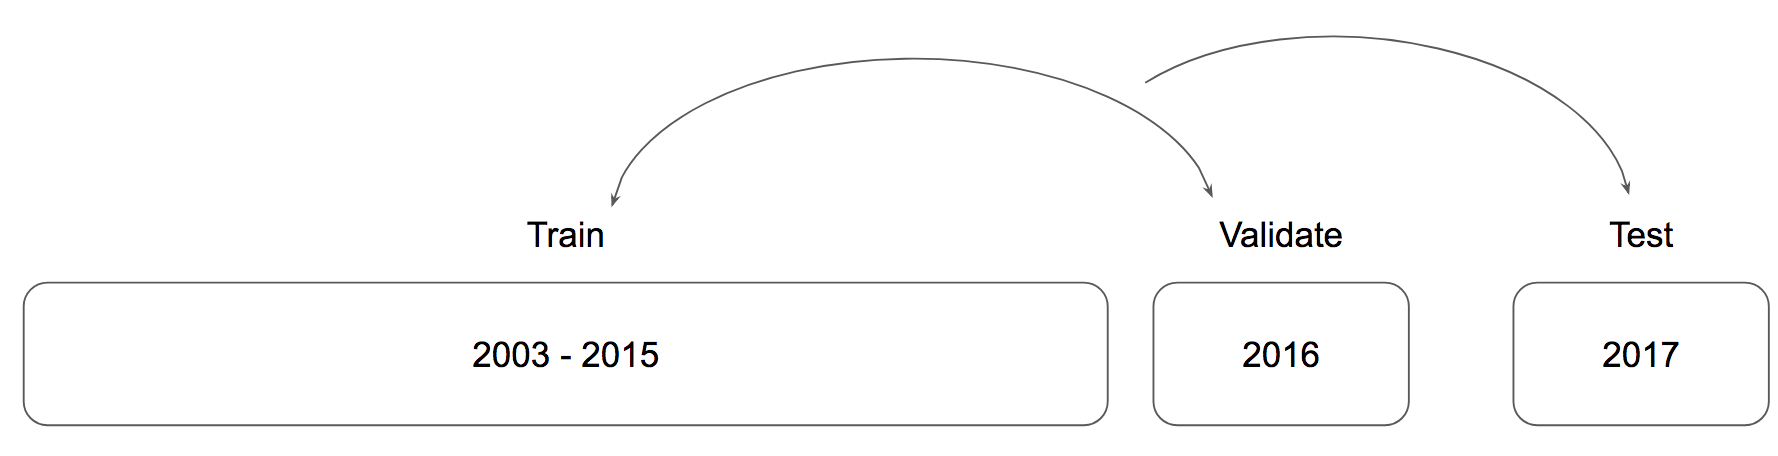
\includegraphics[width=1\linewidth]{Sections/tables and figures/Train Validate Test} \caption{Out-of-time validation}\label{fig:Train Test Validate}
\end{figure}

\subsection{Variable Selection}\label{variable-selection}

For ease of processing and to improve the ability of the model to
generalize into the future, a variable selection step is added to the
modeling process. A Random Forest model is first trained on a 1\%
sub-sample of the modeling data. Variable importance of the resulting
model is calculated using the technique proposed by Friedman (2001),
i.e., for a collection of decision trees \([T_m]_{1}^{m}\):

\begin{flalign*}
  \hat{I_{j}^{2}} = \frac{1}{M} \sum_{m=1}^{M}\hat{I_{j}^{2}}(T_m)
\end{flalign*}

Where influence \(I\) for variable \(j\) is calculated as the sum of
corresponding improvements in squared-error for node tree \(T\). After
calculating variable importance for the model data subset, the variables
are rank-ordered by descending importance. Variables which account for
80\% of the total variable importance are chosen to advance to the model
training round on the full modeling data sets.

\subsection{Evaluation Metrics}\label{evaluation-metrics}

We have chosen evaluation metrics that will allow us to easily compare
the performance of the models against other models with the same outcome
variable. The classification models (Probability of Sale) will be
compared using Area Under the ROC Curve (AUC). The regression models
(Sale Price) will be compared using Root Mean Squared Error (RMSE). Both
evaluation metrics are common for their respective outcome variable
types, and as such will be useful for comparing within model-groups.

\subsubsection{Area Under ROC Curve
(AUC)}\label{area-under-roc-curve-auc}

A classification model typically outputs a probability that a given row
in the data belongs to a group. In the case of binary classification,
the value falls between 0 and 1. There are many techniques for
determining the cut off threshold for classification; a typical method
is to assign anything above a 0.5 into the ``1'' or positive class. An
ROC curve (receiver operating characteristic curve) plots the True
Positive Rate vs.~the False Positive rate at different classification
thresholds; it is a measurement of the performance of a classification
model across all possible thresholds, and therefore sidesteps the need
to arbitrarily assign a cutoff.

Area Under the ROC Curve, or AUC measures the entire two-dimensional
area underneath the ROC curve. It is the integration of the curve from
(0,0) to (1,1), defined as \(AUC = \int_{(0,0)}^{(1,1)} f(x)dx\).

AUC provides a relatively standard measure of performance across all
possible classification thresholds, and can be interpreted as the
probability that the model ranks a random positive example more highly
than a random negative example. A value of 0.5 represents a perfectly
random model, while a value of 1.0 represents a model that can perfectly
discriminate between the two classes. AUC is useful for comparing
classification models against one another because they are both scale
and threshold-invariant.

One of the drawbacks to AUC is that is does not describe the trade-offs
between false positives and false negatives. In certain circumstances, a
false positive might be considerably less desirable than a false
negative, or vice-versa. For our purposes, we rank false positives and
false negatives as equally undesirable outcomes.

\subsubsection{Root Mean Squared Error}\label{root-mean-squared-error}

The Root Mean Squared Error (RMSE) is a common measurement of the
differences between values predicted by a regression model and the
observed values. It is formally defined as
\(RMSE = \sqrt{ \frac{\sum_{1}^{T} (\hat{y}_t - y_t)^2}{T} }\), where
\(\hat{y}\) represents the prediction and \(y\) represents the observed
value at observation \(t\).

Lower RMSE scores are typically more desirable. An RMSE value of 0 would
indicate a perfect fit to the data. RMSE can be difficult to interpret
on its own, however, it is useful for comparing models with similar
outcome variables. In our case, the outcome variables (Sales Price per
Square Foot) are consistent across modeling data sets, and therefore can
be reasonably compared using RMSE.

\section{Results}\label{results}

\subsection{Sale Price Model}\label{sale-price-model}

Using Root Mean Squared Error (RMSE) as an evaluation metric of
predictive power, we find that the Spatial Lag modeling features
consistently outperform the Zip Code features, while the Base modeling
data tends to outperform both, as shown in the following Table (lower
RMSE is better):

\begin{longtable}[]{@{}llll@{}}
\caption{Sale Price Model RMSE For Validation and Test Hold-out
Data}\tabularnewline
\toprule
type & base & zip & spatial lag\tabularnewline
\midrule
\endfirsthead
\toprule
type & base & zip & spatial lag\tabularnewline
\midrule
\endhead
Validation & 280.6 & 298 & 286.2\tabularnewline
Test & 287.8 & 300.6 & 297.9\tabularnewline
\bottomrule
\end{longtable}

Interestingly, both the Spatial Lag modeling data and the Zip Code
modeling data are extensions of the Base data, yet the Base data tends
to generalize to the hold-out data sets better. From this, we make two
observations:

\begin{enumerate}
\def\labelenumi{\arabic{enumi})}
\tightlist
\item
  Building characteristic data, which largely comprises the Base
  modeling data, are the most important for predicting building sale
  price per foot
\item
  The Zip Code and Spatial Lag models are suffering from over-fitting of
  the data, which is limiting their ability to generalize to the
  hold-out samples.
\end{enumerate}

It is possible that the over-fitting issue could be corrected through
hyper-parameter tuning of the algorithms, as well as implementing
stricter variable selection. Despite this, we can still safely conclude
that the Spatial Lag features are superior to the Zip Code features in
terms of predictive power.

Taking a closer look at the data, we find that the models have varying
performance across Building Types and Boroughs. Figure
\ref{fig:RMSE by boro and build type} shows RMSE by Model, faceted by
Borough across the y-axis and Building Type across the x-axis (See Table
2 for a description of building type codes).

\begin{figure}
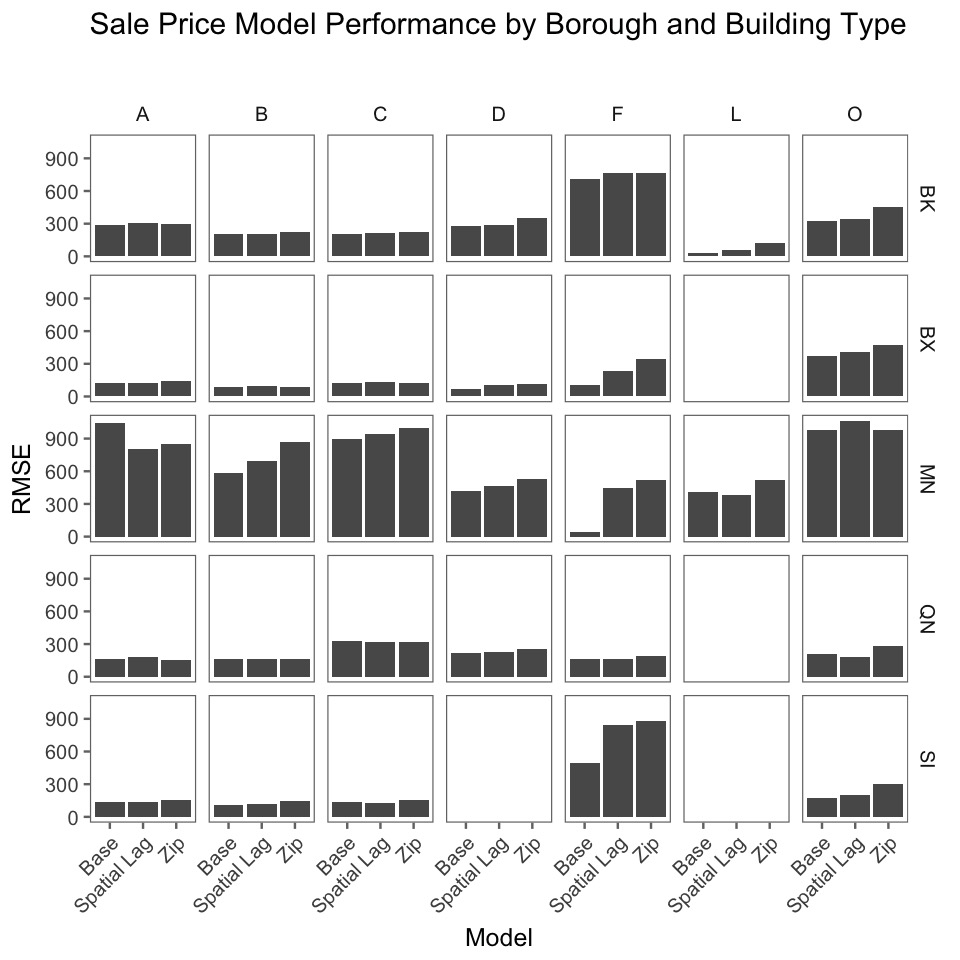
\includegraphics[width=1\linewidth]{Sections/tables and figures/RMSE by boro and build type} \caption{RMSE By Borough and Building Type}\label{fig:RMSE by boro and build type}
\end{figure}

We make the following observations from Figure
\ref{fig:RMSE by boro and build type}:

\begin{itemize}
\tightlist
\item
  The Spatial Lag modeling data outperforms both Base and Zip Code in 6
  cases, notably for Type A buildings (One Family Dwellings) and Type L
  buildings (Lofts) in Manhattan as well as Type O Buildings (Office) in
  Queens
\item
  It is generally harder to predict sale prices in Manhattan than other
  Boroughs
\item
  The ``residential'' building Types A (One Family Dwellings), B (Two
  Family Dwellings), C (Walk Up Apartments) and D (Elevator Apartments)
  have generally lower RMSE scores compared to the non-residential types
\end{itemize}

If we rank the models by performance for each Borough, Building Type
combination, we find that the Spatial Lag models outperform the Zip Code
models in 72\% of cases. Table 9 shows the average ranking by model type
as well as the percent distribution by model type across rankings.

\begin{longtable}[]{@{}lllll@{}}
\caption{Sale Price Model Rankings, RMSE by Borough and Building
Type}\tabularnewline
\toprule
Model Rank & 1 & 2 & 3 & Average Rank\tabularnewline
\midrule
\endfirsthead
\toprule
Model Rank & 1 & 2 & 3 & Average Rank\tabularnewline
\midrule
\endhead
Base & 22.2\% & 9.3\% & 1.9\% & 1.39\tabularnewline
Spatial Lag & 5.6\% & 18.5\% & 9.3\% & 2.11\tabularnewline
Zip & 5.6\% & 5.6\% & 22.2\% & 2.5\tabularnewline
\bottomrule
\end{longtable}

\subsection{Probability of Sale Model}\label{probability-of-sale-model}

Similar to the results found in the Sale Price models, using Area Under
the ROC Curve (AUC) as an evaluation metric, we find the Spatial Lag
model performs better on the hold-out validation data compared to the
Zip Code modeling data, as shown in Table 10. The Base Modeling data
continues to outperform the Spatial Lag and Zip Code modeling data
overall, however, when broken down by Borough and Building Type, some
interesting patterns emerge.

\begin{longtable}[]{@{}llll@{}}
\caption{Probability of Sale Models AUC}\tabularnewline
\toprule
Model AUC & Base & Zip & Spatial Lag\tabularnewline
\midrule
\endfirsthead
\toprule
Model AUC & Base & Zip & Spatial Lag\tabularnewline
\midrule
\endhead
Validation & 0.832 & 0.8292 & 0.8287\tabularnewline
Test & 0.83 & 0.8246 & 0.8279\tabularnewline
\bottomrule
\end{longtable}

Looking at the predictions by the models made on the 2017 validation
hold-out data, we see the Spatial Lag model performs best of any model
for three out of five Boroughs: Manhattan, Bronx and Staten Island
(Table 11).

\begin{longtable}[]{@{}llllll@{}}
\caption{Probability of Sale Models AUC by Borough}\tabularnewline
\toprule
Model & BK & BX & MN & QN & SI\tabularnewline
\midrule
\endfirsthead
\toprule
Model & BK & BX & MN & QN & SI\tabularnewline
\midrule
\endhead
Base & 0.8309 & 0.8288 & 0.7926 & 0.8338 & 0.8336\tabularnewline
Zip & 0.8234 & 0.8215 & 0.7796 & 0.8283 & 0.8281\tabularnewline
Spatial Lag & 0.8257 & 0.8312 & 0.8031 & 0.8327 & 0.8348\tabularnewline
\bottomrule
\end{longtable}

Figure \ref{fig:AUC by boro and build type} shows a breakdown of model
AUC faceted along the x-axis by Building Type and along the y-axis by
Borough. The coloring indicated by how much a model's AUC diverges from
the cell average.

\begin{figure}
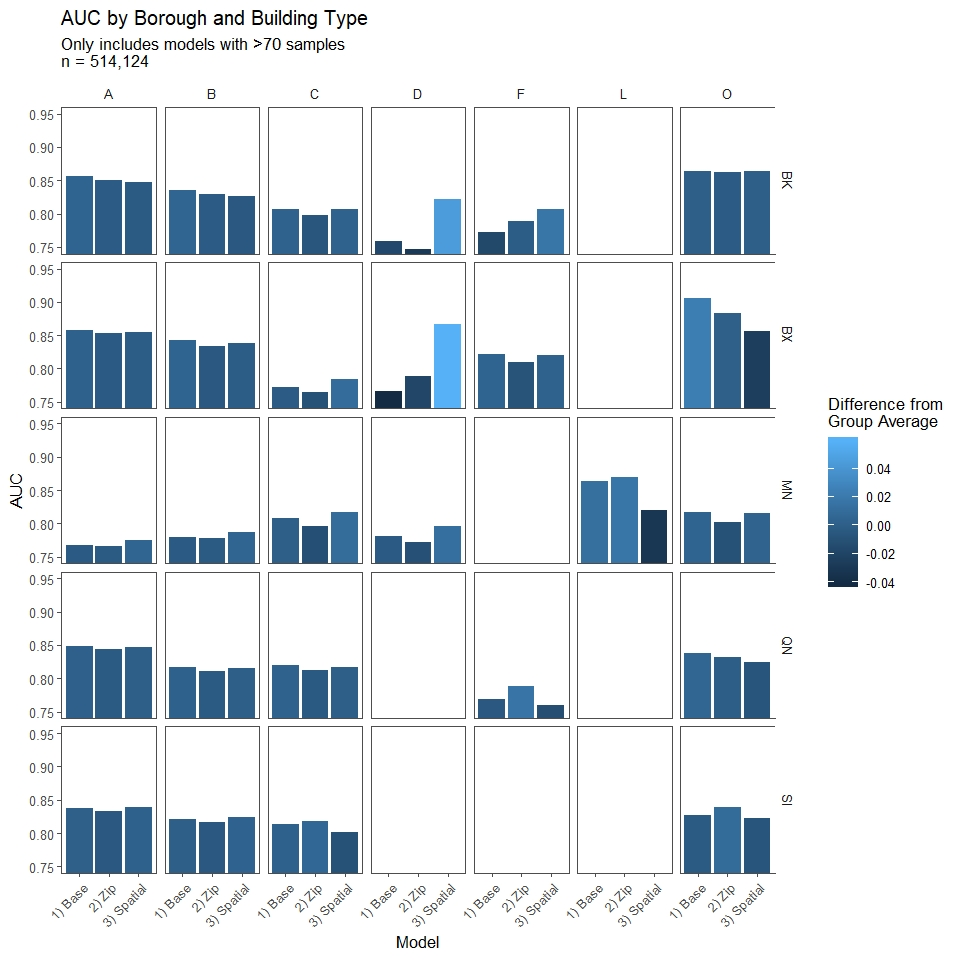
\includegraphics[width=1\linewidth]{Sections/tables and figures/AUC by boro and build type} \caption{AUC By Borough and Building Type}\label{fig:AUC by boro and build type}
\end{figure}

We make the following observations about Figure
\ref{fig:AUC by boro and build type}:

\begin{itemize}
\tightlist
\item
  The Spatial Lag model outperforms all other models for Elevator
  Buildings (Type D), particularly in the Bronx
\item
  The Probability of Sale model tends to perform poorly in Manhattan
  vs.~other Boroughs
\item
  However, the Spatial Lag model performs well in Manhattan for the
  residential building types (A, B, C and D)
\end{itemize}

If we rank model the probability models' performance for each Borough
and Building Type, we see that the Spatial Lag models consistently
outperform the Zip Code models, as shown in Table 12.

\begin{longtable}[]{@{}lllll@{}}
\caption{Distribution and Average Model Rank for Probability of Sale by
AUC across Borough and Building Types}\tabularnewline
\toprule
Model Rank & 1 & 2 & 3 & Average Rank\tabularnewline
\midrule
\endfirsthead
\toprule
Model Rank & 1 & 2 & 3 & Average Rank\tabularnewline
\midrule
\endhead
Base & 16.2\% & 12.0\% & 5.1\% & 2.22\tabularnewline
Spatial Lag & 11.1\% & 13.7\% & 8.5\% & 2.09\tabularnewline
Zip & 6.0\% & 7.7\% & 19.7\% & 1.69\tabularnewline
\bottomrule
\end{longtable}

\section{Conclusions and Future
Research}\label{conclusions-and-future-research}

\subsection{Future Research}\label{future-research}

\begin{itemize}
\tightlist
\item
  Adaptive Bandwidth
\end{itemize}

\subsection{Conclusion}\label{conclusion}

\section{Appendix A: List of Spatial Lag
Features}\label{appendix-a-list-of-spatial-lag-features}

\begin{longtable}[]{@{}l@{}}
\caption{Appendix A: All Spatial Lag Features}\tabularnewline
\toprule
Feature\tabularnewline
\midrule
\endfirsthead
\toprule
Feature\tabularnewline
\midrule
\endhead
Radius Total Sold In Year\tabularnewline
Radius Average Years Since Last Sale\tabularnewline
Radius Res Units Sold In Year\tabularnewline
Radius All Units Sold In Year\tabularnewline
Radius SF Sold In Year\tabularnewline
Radius Total Sold In Year sum over 2 years\tabularnewline
Radius Average Years Since Last Sale sum over 2 years\tabularnewline
Radius Res Units Sold In Year sum over 2 years\tabularnewline
Radius All Units Sold In Year sum over 2 years\tabularnewline
Radius SF Sold In Year sum over 2 years\tabularnewline
Radius Total Sold In Year percent change\tabularnewline
Radius Average Years Since Last Sale percent change\tabularnewline
Radius Res Units Sold In Year percent change\tabularnewline
Radius All Units Sold In Year percent change\tabularnewline
Radius SF Sold In Year percent change\tabularnewline
Radius Total Sold In Year sum over 2 years percent change\tabularnewline
Radius Average Years Since Last Sale sum over 2 years percent
change\tabularnewline
Radius Res Units Sold In Year sum over 2 years percent
change\tabularnewline
Radius All Units Sold In Year sum over 2 years percent
change\tabularnewline
Radius SF Sold In Year sum over 2 years percent change\tabularnewline
Percent Com dist\tabularnewline
Percent Res dist\tabularnewline
Percent Office dist\tabularnewline
Percent Retail dist\tabularnewline
Percent Garage dist\tabularnewline
Percent Storage dist\tabularnewline
Percent Factory dist\tabularnewline
Percent Other dist\tabularnewline
Percent Com basic mean\tabularnewline
Percent Res basic mean\tabularnewline
Percent Office basic mean\tabularnewline
Percent Retail basic mean\tabularnewline
Percent Garage basic mean\tabularnewline
Percent Storage basic mean\tabularnewline
Percent Factory basic mean\tabularnewline
Percent Other basic mean\tabularnewline
Percent Com dist perc change\tabularnewline
Percent Res dist perc change\tabularnewline
Percent Office dist perc change\tabularnewline
Percent Retail dist perc change\tabularnewline
Percent Garage dist perc change\tabularnewline
Percent Storage dist perc change\tabularnewline
Percent Factory dist perc change\tabularnewline
Percent Other dist perc change\tabularnewline
SMA Price 2 year dist\tabularnewline
SMA Price 3 year dist\tabularnewline
SMA Price 5 year dist\tabularnewline
Percent Change SMA 2 dist\tabularnewline
Percent Change SMA 5 dist\tabularnewline
EMA Price 2 year dist\tabularnewline
EMA Price 3 year dist\tabularnewline
EMA Price 5 year dist\tabularnewline
Percent Change EMA 2 dist\tabularnewline
Percent Change EMA 5 dist\tabularnewline
SMA Price 2 year basic mean\tabularnewline
SMA Price 3 year basic mean\tabularnewline
SMA Price 5 year basic mean\tabularnewline
Percent Change SMA 2 basic mean\tabularnewline
Percent Change SMA 5 basic mean\tabularnewline
EMA Price 2 year basic mean\tabularnewline
EMA Price 3 year basic mean\tabularnewline
EMA Price 5 year basic mean\tabularnewline
Percent Change EMA 2 basic mean\tabularnewline
Percent Change EMA 5 basic mean\tabularnewline
SMA Price 2 year dist perc change\tabularnewline
SMA Price 3 year dist perc change\tabularnewline
SMA Price 5 year dist perc change\tabularnewline
Percent Change SMA 2 dist perc change\tabularnewline
Percent Change SMA 5 dist perc change\tabularnewline
EMA Price 2 year dist perc change\tabularnewline
EMA Price 3 year dist perc change\tabularnewline
EMA Price 5 year dist perc change\tabularnewline
Percent Change EMA 2 dist perc change\tabularnewline
Percent Change EMA 5 dist perc change\tabularnewline
SMA Price 2 year basic mean perc change\tabularnewline
SMA Price 3 year basic mean perc change\tabularnewline
SMA Price 5 year basic mean perc change\tabularnewline
Percent Change SMA 2 basic mean perc change\tabularnewline
Percent Change SMA 5 basic mean perc change\tabularnewline
EMA Price 2 year basic mean perc change\tabularnewline
EMA Price 3 year basic mean perc change\tabularnewline
EMA Price 5 year basic mean perc change\tabularnewline
Percent Change EMA 2 basic mean perc change\tabularnewline
Percent Change EMA 5 basic mean perc change\tabularnewline
\bottomrule
\end{longtable}

\section*{References}\label{references}
\addcontentsline{toc}{section}{References}

\hypertarget{refs}{}
\hypertarget{ref-Almanie2015}{}
Almanie, R.; Lor, T.; Mirza. 2015. ``Crime Prediction Based on Crime
Types and Using Spatial and Temporal Criminal Hotspots.''
\emph{International Journal of Data Mining \& Knowledge Management
Process (IJDKP)} 5 (4).

\hypertarget{ref-antipov12}{}
Antipov, Evgeny A., and Elena B. Pokryshevskaya. 2012. ``Mass Appraisal
of Residential Apartments: An Application of Random Forest for Valuation
and a Cart-Based Approach for Model Diagnostics.'' \emph{Expert Systems
with Applications}.

\hypertarget{ref-Pollack2010}{}
Barry Bluestone \& Chase Billingham, Stephanie Pollack \&. 2010.
``Maintaining Diversity in America's Transit-Rich Neighborhoods: Tools
for Equitable Neighborhood Change.'' \emph{New England Community
Developments, Federal Reserve Bank of Boston}, 1--6.

\hypertarget{ref-Breiman2001}{}
Breiman, L. 2001. ``Random Forests.'' \emph{Machine Learning} 45 (1):
5--32.

\hypertarget{ref-Chapple2009}{}
Chapple, Karen. 2009. ``Mapping Susceptibility to Gentrification: The
Early Warning Toolkit.'' \emph{Berkeley, CA: Center for Community
Innovation.}

\hypertarget{ref-Chapple2016}{}
Chapple, Miriam, Karen; Zuk. 2016. ``Forewarned: The Use of Neighborhood
Early Warning Systems for Gentrification and Displacement.''
\emph{Cityscape: A Journal of Policy Development and Research} 18 (3).

\hypertarget{ref-Clay1979}{}
Clay, Phillip L. 1979. \emph{Neighborhood Renewal: Middle-Class
Resettlement and Incumbent Upgrading in American Neighborhoods}.
Lexington Books.

\hypertarget{ref-Dietzell2014}{}
Dietzell, Nicole; Schäfers, Marian Alexander; Braun. 2014.
``Sentiment-Based Commercial Real Estate Forecasting with Google Search
Volume Data.'' \emph{Journal of Property Investment \& Finance,} 32 (6):
540--69.

\hypertarget{ref-Dreier2004}{}
Dreier, John; Swanstrom, Peter; Mollenkopf. 2004. \emph{Place Matters:
Metropolitics for the Twenty-First Century.} University Press of Kansas.

\hypertarget{ref-Springer2017}{}
d'Amato, Tom, Maurizio; Kauko, ed. 2017. \emph{Advances in Automated
Valuation Modeling}. Springer International Publishing.

\hypertarget{ref-Eckert1990}{}
Eckert, J. K. 1990. \emph{Property Appraisal and Assessment
Administration}. Chicago, IL.: International Association of Assessing
Officers.

\hypertarget{ref-Fotheringham2015}{}
Fotheringham, R; Yao, A.S.; Crespo. 2015. ``Exploring, Modelling and
Predicting Spatiotemporal Variations in House Prices.'' \emph{The Annals
of Regional Science} 54.

\hypertarget{ref-Friedman2001}{}
Friedman, Jerome H. 2001. ``Greedy Function Approximation: A Gradient
Boosting Machine.'' \emph{The Annals of Statistics} 29 (5): 1189--1232.

\hypertarget{ref-Fu2014}{}
Fu, Yanjie; et al. 2014. \emph{Exploiting Geographic Dependencies for
Real Estate Appraisal: A Mutual Perspective of Ranking and Clustering}.
Proceedings of the 20th ACM SIGKDD international conference on Knowledge
discovery; data mining.

\hypertarget{ref-Geltner2017}{}
Geltner, David, and Alex Van de Minne. 2017. ``Do Different Price Points
Exhibit Different Investment Risk and Return Commercial Real Estate.''
Real Estate Research Institute.

\hypertarget{ref-Guan2014}{}
Guan, Jian, Donghui Shi, Jozef M. Zurada, and Alan S. Levitan. 2014.
``Analyzing Massive Data Sets: An Adaptive Fuzzy Neural Approach for
Prediction, with a Real Estate Illustration.'' \emph{Journal of
Organizational Computing and Electronic Commerce} 24 (1). Taylor \&
Francis: 94--112.
doi:\href{https://doi.org/10.1080/10919392.2014.866505}{10.1080/10919392.2014.866505}.

\hypertarget{ref-Helbich2013}{}
Helbich, et al., Marco. 2013. ``Boosting the Predictive Accuracy of
Urban Hedonic House Price Models Through Airborne Laser Scanning.''
\emph{Computers, Environment and Urban Systems} 39: 81--92.

\hypertarget{ref-Johnson2007}{}
Johnson, Ken, Justin Benefield, and Jonathan Wiley. 2007. ``The
Probability of Sale for Residential Real Estate.'' \emph{Journal of
Housing Research} 16 (2): 131--42.
doi:\href{https://doi.org/10.5555/jhor.16.2.0234g75800h5k8x6}{10.5555/jhor.16.2.0234g75800h5k8x6}.

\hypertarget{ref-Kontrimasa2011}{}
Kontrimasa, Antanas, Vilius; Verikasb. 2011. ``The Mass Appraisal of the
Real Estate by Computational Intelligence.'' \emph{Applied Soft
Computing}.

\hypertarget{ref-Koschinsky2012}{}
Koschinsky, J. et al. 2012. ``The Welfare Benefit of a Home's Location:
An Empirical Comparison of Spatial and Non-Spatial Model Estimates.''
\emph{Journal of Geographical Systems} 10109.

\hypertarget{ref-Lees2008}{}
Lees, Tom; Wyly, Loretta; Slater. 2008. ``Gentrification.'' \emph{Growth
and Change} 39 (3): 536--39.
doi:\href{https://doi.org/10.1111/j.1468-2257.2008.00443.x}{10.1111/j.1468-2257.2008.00443.x}.

\hypertarget{ref-Miller2015}{}
Miller, J.; Aspinall, J.; Franklin. 2007. ``Incorporating Spatial
Dependence in Predictive Vegetation Models.'' \emph{Ecological
Modelling} 202 (3): 225--42.

\hypertarget{ref-Park2015}{}
Park, Jae Kwon, Byeonghwa; Bae. 2015. ``Using Machine Learning
Algorithms for Housing Price Prediction: The Case of Fairfax County,
Virginia Housing Data.'' \emph{Expert Systems with Applications} 42 (6):
2928--34.

\hypertarget{ref-Pivo2011}{}
Pivo, Gary, and Jeffrey D. Fisher. 2011. ``The Walkability Premium in
Commercial Real Estate Investments.'' \emph{Real Estate Economics} 39
(2): 185--219.
doi:\href{https://doi.org/10.1111/j.1540-6229.2010.00296.x}{10.1111/j.1540-6229.2010.00296.x}.

\hypertarget{ref-Quintos2013}{}
Quintos, Carmela. 2013. ``Estimating Latent Effects in Commercial
Property Models.'' \emph{Journal of Property Tax Assessment \&
Administration} 12 (2).

\hypertarget{ref-Rafiei2016}{}
Rafiei, Hojjat, Mohammad Hossein; Adeli. 2016. ``A Novel Machine
Learning Model for Estimation of Sale Prices of Real Estate Units.''
\emph{Journal of Construction Engineering and Management} 142 (2).

\hypertarget{ref-Reardon2011}{}
Reardon, Kendra, Sean F.; Bischoff. 2011. ``Income Inequality and Income
Segregation.'' \emph{American Journal of Sociology}.

\hypertarget{ref-Schernthanner2016}{}
Schernthanner H., Gonschorek J., Asche H. 2016. ``Spatial Modeling and
Geovisualization of Rental Prices for Real Estate Portals.''
\emph{Computational Science and Its Applications} 9788.

\hypertarget{ref-Silverherz1936}{}
Silverherz, J. D. 1936. ``The Assessment of Real Property in the United
States.'' \emph{Albany: J.B. Lyon Co. Printers}.

\hypertarget{ref-Smith1979}{}
Smith, Neil. 1979. ``Toward a Theory of Gentrification a Back to the
City Movement by Capital, Not People.'' \emph{Journal of the American
Planning Association} 45 (4). Routledge: 538--48.
doi:\href{https://doi.org/10.1080/01944367908977002}{10.1080/01944367908977002}.

\hypertarget{ref-urban2016}{}
Solomon Greene, Molly Scott, Rolf Pendall, and Serena Lei. 2016. ``Open
Cities: From Economic Exclusion to Urban Inclusion.'' \emph{Urban
Institue Brief}, June. Urban Institue Brief.

\hypertarget{ref-Turner2001}{}
Turner, Margery Austin, and Christopher Snow. 2001. \emph{Leading
Indicators of Gentrification in d.C. Neighborhoods}.

\hypertarget{ref-Watson2009}{}
Watson, Tara. 2009. ``Inequality and the Measurement of Residential
Segregation by Income in American Neighborhoods.'' \emph{Review of
Income and Wealth}.

\hypertarget{ref-Zuk2015}{}
Zuk, Miriam; et al. 2015. ``Gentrification, Displacement and the Role of
Public Investment: A Literature Review.''


\end{document}
